\chapter*{Programme officiel}

\section*{Programme officiel}

Lors de la navigation sur le Web, les internautes interagissent avec leur machine par le biais des pages Web.

L'Interface Homme-Machine (IHM) repose sur la gestion d'événements associés à des éléments graphiques munis de méthodes algorithmiques.

La compréhension du dialogue client-serveur déjà abordé en classe de seconde est consolidée, sur des exemples simples, en identifiant les requêtes du client, les calculs puis les réponses du serveur traitées par le client.

Il ne s'agit pas de décrire exhaustivement les différents éléments disponibles, ni de développer une expertise dans les langages qui permettent de mettre en œuvre le dialogue tels que PHP ou JavaScript.

{\centering\begin{tabular}{|L{3cm}|L{5.5cm}|L{6cm}|}\hline
\cellcolor{bo}\bfseries\textcolor{white}{Contenus}&
\cellcolor{bo}\bfseries\textcolor{white}{Capacités attendues}&
\cellcolor{bo}\bfseries\textcolor{white}{Commentaires}\\ \hline
Modalités de l'interaction entre l'homme et la machine

Événements
&
Identifier les différents composants graphiques permettant d'interagir avec une application Web.

Identifier les événements que les fonctions associées aux différents composants graphiques sont capables de traiter.
&
Il s'agit d'examiner le code HTML d'une page comprenant des composants graphiques et de distinguer ce qui relève de la description des composants graphiques en HTML de leur comportement (réaction aux événements) programmé par exemple en JavaScript.\\ \hline
Interaction avec l'utilisateur dans une page Web
&
Analyser et modifier les méthodes exécutées lors d'un clic sur un bouton d'une page Web.
&
\\ \hline
Interaction client-serveur.

Requêtes HTTP, réponses du serveur
&
Distinguer ce qui est exécuté sur le client ou sur le serveur et dans quel ordre.

Distinguer ce qui est mémorisé dans le client et retransmis au serveur.

Reconnaître quand et pourquoi la transmission est chiffrée.
&
Il s'agit de faire le lien avec ce qui a été vu en classe de seconde et d'expliquer comment on peut passer des paramètres à un site grâce au protocole HTTP.\\ \hline
Formulaire d'une page Web
&
Analyser le fonctionnement d'un formulaire simple.

Distinguer les transmissions de paramètres par les requêtes POST ou GET.
&
Discuter les deux types de requêtes selon le type des valeurs à transmettre et/ou leur confidentialité.\\ \hline
\end{tabular}\par}


\chapter{Les langages : HTML, CSS et JavaScript}

\section{Balises HTML}

\Cours{{\bfseries HTML} : HyperText Markup Language

C'est un langage de description de page web.

Un fichier HTML est un fichier texte, qui utilise des \emph{balises} pour définir la structure et le contenu d'une page Web (indépendamment de la façon de l'afficher).
}

Tout fichier HTML en français, devrait contenir au moins les dix lignes proposées ci-dessous.

\begin{multicols}{2}
Les éléments commençant et terminant par les chevrons \mintinline{html}{<} et \mintinline{html}{>} sont des \emph{balises}.

\begin{itemize}
	\item \mintinline{html}{<balise>} est une balise ouvrante,
	\item \mintinline{html}{</balise>} une balise fermante et
	\item \mintinline{html}{<balise />} une balise auto-fermante.
\end{itemize}

Toute balise ouverte doit être fermée.

Pour afficher les caractères < et > on utilise les entités : \mintinline{html}{&lt;} et \mintinline{html}{&gt;}.

\begin{minted}{HTML}
<!DOCTYPE html>
<html lang="fr">
  <head>
    <meta charset="UTF-8" />
    <title><!-- Un titre --></title>
  </head>
  <body>
    <!-- Du contenu -->
  </body>
</html>
\end{minted}
\end{multicols}

Quelques balises << indispensables >> :

\begin{multicols}{2}
\begin{tabular}{|ll|}
\hline
\multicolumn{2}{|c|}{Structurer le contenu}\\
\hline
\mintinline{html}{<h1>} & Titre principal \\
\mintinline{html}{<h2>} & Titre secondaire \\
\multicolumn{1}{|c}{\vdots} & \multicolumn{1}{c|}{\vdots} \\
\mintinline{html}{<h6>} & Plus petit sous-titre\\
\mintinline{html}{<p>}  & Paragraphe\\
\mintinline{html}{<br />} & Retour à la ligne\\
\hline
\end{tabular}


\begin{minted}[breaklines]{HTML}
<h1>Langage HTML</h1>

<h2>Les balises</h2>

<p>Ce sont les éléments commençant par
  &lt; et terminant par &gt;.<br />
  Exemple : &lt;br /&gt;</p>
\end{minted}
\end{multicols}

Les balises \mintinline{html}{<p>} et \mintinline{html}{<h1>}, ... sont de type \emph{block} : leur contenu prend toute la largeur disponible sur la page. Elles provoquent donc automatiquement un passage à la ligne. La balise générique de ce type est : \mintinline{html}{<div>}

\medskip

\begin{multicols}{2}
\begin{tabular}{|ll|}
\hline
\multicolumn{2}{|c|}{Faire des liens}\\
\hline
\mintinline{html}{<a>} & Lien hypertexte\\
\mintinline{html}{<img />} & Inclure une image \\
\hline
\end{tabular}


\begin{minted}[breaklines]{HTML}
<p>Cliquez l'image ci-dessous pour 
  aller sur mon site.<br />
  <a href="www.monsite.fr">
    <img src="../images/logo.png" />
  </a></p>
\end{minted}
\end{multicols}

Les balises \mintinline{html}{<a>} et \mintinline{html}{<img />}, ... sont de type \emph{inline} : leur contenu prend seulement la place dont il a besoin (pas de passage à la ligne). La balise générique de ce type est : \mintinline{html}{<span>}

\medskip

\begin{multicols}{2}
\begin{tabular}{|ll|}
\hline
\multicolumn{2}{|c|}{Faire une liste}\\
\hline
\mintinline{html}{<ul>} & Liste non numérotée\\
\mintinline{html}{<ol>} & Liste numérotée\\
\mintinline{html}{<li>} & Élément d'une liste\\
\hline
\end{tabular}


\begin{minted}{HTML}
<ul>
  <li> les balises <em>block</em></li>
  <li> les balises <em>inline</em></li>
</ul>
\end{minted}
\end{multicols}

La  balise \mintinline{html}{<em>} permet de mettre du texte en valeur (emphase). Il existe beaucoup d'autres balises dont on trouve facilement des listes et descriptions par exemple sur \href{https://www.w3schools.com/}{www.w3schools.com/}.

\section{Éléments de CSS}

\Cours{{\bfseries CSS} : Cascading Style Sheets

Un fichier CSS, appelé souvent << feuille de style >> est un fichier texte permettant de décrire la manière d'afficher ce qui est défini dans une page HTML.
}

Pour lier la feuille de style \texttt{style.css}, on inclut un lien dans l'entête de la page :

\begin{minted}{HTML}
<head>
  <!-- entête -->
  <link rel="stylesheet" type="text/css" href="chemin/style.css"/>
</head>
\end{minted}



\begin{multicols}{2}

La feuille de style permet alors de décrire l'affichage de chaque balise.

Par exemple on peut préciser la couleur d'un élément par un nom (dans une liste prédéfinie), par ses composantes \texttt{rgb} ou par son code hexadécimal.

\begin{minted}{CSS}
/* ---- généralités --- */
body {
  background-color : AliceBlue;
  color : rgb(128,128,255);
  border-color : #A1BBFF;
  border-style : solid;
}
\end{minted}
\end{multicols}

\medskip

Pour associer un style particulier à une seule balise du fichier HTML, on associe à cette balise un identifiant unique par le sélecteur \mintinline{html}{id} :

\begin{multicols}{2}
\begin{minted}{HTML}
<p id="particulier">Ce paragraphe 
  est traité de manière très 
  particulière.</p>
  
<p>Celui-ci ne change pas </p>

\end{minted}

\begin{minted}{CSS}
/* ---- cas particulier --- */
#particulier {
  text-align : center;
  font-size : 1.5vw; /* ou px ou em*/
}
\end{minted}
\end{multicols}

Pour associer un style particulier à plusieurs balises (éventuellement différentes) du fichier HTML, on associe à ces balises une classe commune par le sélecteur \mintinline{html}{class} :

\begin{multicols}{2}
\begin{minted}{HTML}
<h2 class="important"> Ce titre est 
important.</h2>
<p> Voila pourquoi </p>
<p class="important">Ce paragraphe 
  est important.</p>
\end{minted}
\begin{minted}{CSS}
/* ---- classe --- */
.important {
  text-decoration : underline;
  font-weight : bold;
}
\end{minted}

\end{multicols}

On peut préciser le style d'une balise selon son état. En particulier pour les liens :

\begin{multicols}{2}
\begin{minted}{HTML}
Pour la définition, voir le
<a href="mapage.html#chapitre1">
chapitre 1</a>.
\end{minted}

\begin{minted}{CSS}
/* ---- états --- */
a:link { color: red; }
a:visited { color: green; }
a:hover { color: hotpink; }
a:active { color: blue; }
\end{minted}

\end{multicols}

L'état \mintinline{html}{:hover}, en particulier, est utilisable pour les autres balises. 

\section{Notions de JavaScript}

\Cours{{\bfseries JavaScript}

C'est un langage de programmation, interprété par les navigateurs web.}

\mintinline{HTML}{<script>/* instructions */</script>} permet d'inclure des instructions JavaScript dans un document html. Mais on privilégie l'inclusion de fichiers : \mintinline{HTML}{<script src="script.js"></script>} pour garder la lisibilité de structure HTML. On peut, en sortie,  écrire dans 
\begin{itemize}
	\item la console du navigateur avec la fonction \mintinline{js}{console.log()} ;
	\item le document en train de s'afficher avec la fonction \mintinline{js}{document.write()} ;
	\item une fenêtre d'alerte avec la fonction \mintinline{js}{window.alert()} ;
	\item un élément de la page déjà affiché par son attribut \mintinline{js}{innerHTML}.
\end{itemize} 

\begin{multicols}{2}

\begin{minted}{HTML}
<!DOCTYPE html>
<html lang="fr">
  <head>
    <meta charset="UTF-8" />
    <title>Tests de sorties</title>
  </head>
  <body>
    <p>Paragraphe 1</p>
    <p id="fin">Paragraphe 2</p>
    <script src="script.js"></script>
  </body>
</html>
\end{minted}

Les instructions JavaScript, comme le contenu HTML, est interprété dans l'ordre des lignes.

\begin{minted}{js}
/* Fichier script.js*/
document.write("<strong>FIN</strong>");
var e = document.getElementById("FIN")
e.innerHTML = "Dernier paragraphe.";
console.log("Modification : OK.")
window.alert("Paragraphe 2 modifié !");
\end{minted}

\noindent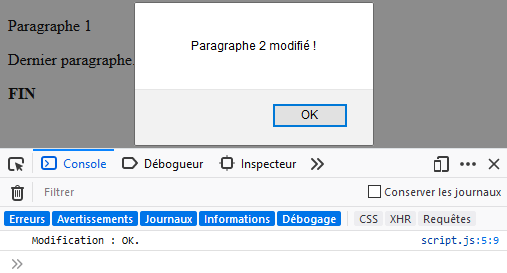
\includegraphics[width=\linewidth]{images/jslog.png}

\end{multicols}

Une fois un élément de la page HTML portant un identifiant récupéré par la fonction \mintinline{JS}{document.getElementById()}, on peut :

\begin{itemize}
	\item modifier ses attributs : \mintinline{JS}{e.setAttribute("attribut", "valeur");},
	\item supprimer ses attributs : \mintinline{JS}{e.removeAttribute("attribut");},
	\item agir sur sa classe (donc son style) : \mintinline{JS}{e.className = 'classe';}.
\end{itemize}

Et comme c'est un langage de programmation, on a les structures habituelles :

\begin{multicols}{3}\centering
Variables

\vspace{-2ex}
\begin{minted}[fontsize=\footnotesize]{js}
var x, y;
x = 7;
y = 7 ** 2;
\end{minted}

Appels de fonction

\vspace{-2ex}
\begin{minted}[fontsize=\footnotesize]{js}
function double(x) {
  return 2 * x;
}
console.log(double(7));
\end{minted}

Boucles bornées

\vspace{-2ex}
\begin{minted}[fontsize=\footnotesize]{js}
for (var i=0; i<9; i++) {
  console.log(i);
}
\end{minted}

Boucles non bornées

\vspace{-2ex}
\begin{minted}[fontsize=\footnotesize]{js}
var n = 0;
while (n < 3) {
  n++; console.log(n);
}
\end{minted}

Conditionnelles

\vspace{-2ex}
\begin{minted}[fontsize=\footnotesize]{js}
if (x < y) {
  console.log("ok");
} else {
  console.log("!!");
}
\end{minted}

(Chaque instruction étant terminée par un point-virgule.)
\end{multicols}

\section{Réaction aux événements}

\Cours{{\bfseries Événement}

Un événement est un changement d'état de l'environnement. Il peut être créé par l'utilisateur (avec le clavier, la souris...), par le document lui-même (fin de chargement d'une image, ou de la page...) ou encore par l'exécution d'un code JavaScript.}

\Cours{{\bfseries Gestionnaire d'événements}

Un événement une fois créé va se propager aux différents niveaux de définition de la page (document, html, body, jusqu'à l'élément cible et retour). Le rôle d'un gestionnaire d'événement est de l'intercepter et de réagir (souvent par un appel à une fonction JavaScript).}

Un gestionnaire d'événement peut être directement placé dans une balise HTML :

\vspace{-2ex}
\begin{minted}{html}
<!-- Dans l'en-tête -->
<script src="script.js"></script>
<link rel="stylesheet" type="text/css" href="style.css"/>
<!-- Dans le corps -->
<spam onmouseover="rouge(event)" onmouseout="noir(event)">Survolez-moi</spam>
\end{minted}

\vspace{-2ex}
\begin{multicols}{2}
avec dans \texttt{style.css} :

\vspace{-2ex}
\begin{minted}{css}
.noir { 
  color : black; 
}
.rouge { 
  color : red; 
}
\end{minted}


et dans \texttt{script.js} :

\vspace{-2ex}
\begin{minted}{css}
function rouge(e) {
  e.target.className = 'rouge'
} 
function noir(e) {
  e.target.className = 'noir'
}
\end{minted}

\end{multicols}

Dans cet exemple, passer sur les mots \texttt{Survolez-moi} ou les quitter avec la souris génère un événement. Il est capté par \mintinline{JS}{onmouseover} ou \mintinline{JS}{onmouseout} qui le transmettent aux fonctions JavaScript qui agissent sur le style graphique de ces mots. On peut citer de plus :

\begin{itemize}
	\item \mintinline{JS}{onchange} : un élément a changé.
	\item \mintinline{JS}{onclick} :  l'utilisateur a cliqué sur un élément.
	\item \mintinline{JS}{onkeydown} :  l'utilisateur a appuyé sur une touche.
	\item \mintinline{JS}{onload} : la page a fini d'être chargée.
\end{itemize}

L'élément cliquable par excellence est le bouton :

\vspace{-2ex}
\begin{minted}{html}
<button type="button" onclick="alert(event.target.innerHTML)">GO !</button>
\end{minted}

\chapter{Client, serveur et protocole HTTP}

\section{Modèle client/serveur}

Pour présenter ce modèle, on se place dans un réseau et sous le protocole de communication TCP/IP (voir partie Architectures matérielles). On ne considère que deux ordinateurs en train de communiquer.

\Cours{{\bfseries Modèle client/serveur}
\begin{multicols}{2}
C'est un modèle de communication dissymétrique entre deux ordinateurs sur un réseau.

\begin{itemize}
	\item Le client envoie une requête au serveur.
	\item Le serveur répond au client.
\end{itemize}

\begin{tikzpicture}
\node[](O){\ordinateur};\node[below]at(O.south){\small Client};
\node[right=2cm](S)at(O.east){\serveur};\node[below]at(S.south){\small Serveur};
\draw[-latex]($(O.east)+(0,0.3cm)$)--($(S.west)+(0,0.3cm)$)node[midway, above]{\small requête};
\draw[-latex]($(S.west)-(0,0.3cm)$)--($(O.east)-(0,0.3cm)$)node[midway, below]{\small réponse};
\end{tikzpicture}
\end{multicols}}

Voici une proposition minimaliste d'un client et d'un serveur en Python.

\begin{minted}{python}
import socket

hote = "localhost"
port = 12800

connexion = socket.socket(socket.AF_INET, socket.SOCK_STREAM)
connexion.connect((hote, port))
print("Connexion établie avec le serveur sur le port",port)

msg_a_envoyer = input("> ").encode()
connexion.send(msg_a_envoyer)
msg_recu = connexion.recv(1024)
print(msg_recu.decode())

connexion.close()
\end{minted}
\begin{tikzpicture}[overlay, xshift = 15cm, yshift=6.5cm]
\node[](O){\ordinateur};\node[below]at(O.south){\small Client};
\end{tikzpicture}

\vspace{-3ex}
On utilise un socket pour spécifier, selon le protocole TCP/IP, l'adresse du serveur et son port de communication. Ici, le serveur test est sur le même ordinateur que le client (\mintinline{python}{"localhost"}) et utilise le port 12800.

On peut observer les trois actions principales d'un client.

\begin{enumerate}
	\item La connexion avec le serveur (lignes 7)
	\item L'échange de messages (lignes 11 et 12)
	\item La déconnexion du serveur (ligne 15)
\end{enumerate}

Les messages échangés sont du domaine des applications (plus haute couche du modèle). Cela concerne par exemple les pages html (protocoles http ou https), l'échange de fichiers (protocole ftp) ou de mails (protocole smtp)...

\medskip

La requête (message envoyé au serveur) peut contenir des informations que le serveur traitera pour envoyer une réponse adaptée et personnelle à l'utilisateur (on parle de site dynamique, à opposer aux sites statiques qui ont un contenu indépendant de l'utilisateur). Ce traitement se fait à l'aide de programmation (avec différents langages : php ou python ou ...).

La réponse peut également contenir des éléments dynamiques pour l'utilisateur (en JavaScript par exemple).

\begin{minted}{python}
import socket

hote = ''
port = 12800

serveur = socket.socket(socket.AF_INET, socket.SOCK_STREAM)
serveur.bind((hote, port))
serveur.listen(5)
print("Le serveur écoute sur le port",port)

client, infos = serveur.accept()

msg_recu = client.recv(1024)
print(msg_recu.decode())
client.send(b"5 / 5")

client.close()
serveur.close()
\end{minted}
\begin{tikzpicture}[overlay, xshift = 15cm, yshift=7.5cm]
\node[](O){\serveur};\node[below]at(O.south){\small Serveur};
\end{tikzpicture}

\vspace{-2ex}
On peut observer les quatre actions principales d'un serveur.

\begin{enumerate}
	\item L'attente d'une connexion avec le client (lignes 8)
	\item La connexion avec un client (ligne 11)
	\item L'échange de messages (lignes 13 et 15)
	\item La déconnexion du client (ligne 17)
\end{enumerate}

Les réponses ne sont en général pas générées directement par le serveur. Il peut lui-même faire des requêtes à une base de données, récupérer des modèles et/ou demander à un autre programme de générer la vue à transmettre au client (le Modèle-Vue-Contrôleur : MVC).

\section{Protocole HTTP}

\Cours{{\bfseries HTTP} (HyperText Transfert Protocol)

C'est un protocole de la couche application (la plus haute sur modèle TCP/IP) permettant la demande et l'envoi de ressources. Il a été conçu pour la communication entre un navigateur web (client) et un serveur web.
}

Pour les premiers tests, on utilisera le serveur HTTP à l'adresse \href{http://httpbin.org/}{http://httpbin.org/} qui renvoie en écho les données utilisées dans la requête.

\subsection{Requête HTTP}

Une requête HTTP est de la forme :

\begin{minted}{text}
VERBE URI HTTP/X.X
En-têtes
Corps
\end{minted}

\begin{itemize}
	\item Le \mintinline{text}{VERBE} est le plus souvent \mintinline{text}{GET} pour \emph{obtenir} une ressource, ou \mintinline{text}{POST} pour \emph{envoyer}, par exemple, le contenu d'un formulaire.
	\item L'\mintinline{text}{URI} (Uniform Ressource Identifier) est l'URL (Uniform Ressource Locator) complété pour préciser la ressource visée à cette adresse.
	\item \mintinline{text}{HTTP/X.X} indique la version du protocole : \texttt{HTTP/1.1}
	\item \mintinline{text}{En-tête} (optionnel) permet de préciser la ressource et le comportement du client/serveur.
	
	Chaque ligne est composée d'un nom, de deux points \mintinline{text}{:} et de valeurs.

    Par exemple : \pythoninline{Accept-Language: fr,fr-FR;q=0.8,en-US;q=0.5,en;q=0.3}
	\item \mintinline{text}{Corps} contient des données précisant la demande de ressource. Cette partie est vide pour la méthode GET (qui peut tout de même préciser sa demande via l'URI).
\end{itemize}

En Python, on utilisera la bibliothèque \pythoninline{requests} (à installer).

Code minimal pour une requête GET, avec précisions au bout de l'URL :

\vspace{-2ex}
\begin{minted}{python}
import requests

ressource = requests.get('http://httpbin.org/get?test=True&valeur=2')
print(ressource.text)
\end{minted}

Affiche :

\vspace{-2ex}
\begin{minted}{text}
{
  "args": {
    "test": "True", 
    "valeur": "2"
  }, 
  "headers": {
    "Accept": "*/*", 
    "Accept-Encoding": "gzip, deflate", 
    "Host": "httpbin.org", 
    "User-Agent": "python-requests/2.22.0"
  }, 
  "origin": "xxx.xxx.xxx.xxx, xxx.xxx.xxx.xxx", 
  "url": "https://httpbin.org/get?test=True&valeur=2"
}
\end{minted}

On peut observer quelques éléments d'en-tête et que les précisions en bout d'URL ont bien été captées.

\medskip

Code minimal pour une requête POST, avec envoi de données encodées comme si elles venaient d'un formulaire HTML :

\vspace{-2ex}
\begin{minted}{python}
import requests

donnees = {'clef1': 'valeur1', 'clef2': 'valeur2'}
ressource = requests.post('http://httpbin.org/post', data = donnees)
print(ressource.text)
\end{minted}

Les données ont bien été transmises comme venant d'un formulaire :


\vspace{-2ex}
\begin{minted}{text}
{
  "args": {}, 
  "data": "", 
  "files": {}, 
  "form": {
    "test": "True", 
    "valeur": "2"
  }, 
  ...
\end{minted}

Si ces données ne sont pas trop importantes, elles peuvent être envoyées par la méthode GET mais seront visibles dans l'URI. Celles transmises par la méthode POST ne le sont pas, mais restent transmises en clair, dans le corps de la requête. Si on souhaite une transmission sécurisée, il faudra en plus utiliser un système de chiffrement.

\medskip

{\bfseries Pour aller plus loin :} D'autres façons de transmettre les données sont possibles.

Par exemple en JSON :

\vspace{-2ex}
\begin{minted}{python}
import requests
import json

donnees = {'test': True, 'valeur': 2}
donneesJSON = json.dumps(donnees)
ressource = requests.post('http://httpbin.org/post', data = donneesJSON)
\end{minted}

Ou sinon directement en chaîne de caractères :

\vspace{-2ex}
\begin{minted}{python}
import requests

donnees = "Ma structure"
ressource = requests.post('http://httpbin.org/post', data = donnees)
\end{minted}



\subsection{Réponse HTTP}

Une réponse HTTP a la même forme qu'une requête sauf pour la première ligne :

\begin{minted}{text}
HTTP/X.X CODE MESSAGE
En-têtes
Corps
\end{minted}

\begin{itemize}
	\item \pythoninline{CODE} et  \pythoninline{MESSAGE} indiquent le statut de la communication.
	
	Exemples : \mintinline{text}{200 OK} ou le fameux \mintinline{text}{404 Not Found}. Voir \href{https://httpstatuses.com/}.{https://httpstatuses.com/}
	
	On peut obtenir le CODE d'une réponse par : \pythoninline{ressource.status_code}.
	\item On peut obtenir l'\mintinline{text}{en-tête} par : \pythoninline{ressource.headers} (donne un dictionnaire).
	\item On peut obtenir le \mintinline{text}{corps} au format texte par : \pythoninline{ressource.text}.
	      
	      En précisant \emph{avant} l'encodage si besoin : \pythoninline{ressource.encoding = 'utf-8'}.
	
	\item On peut obtenir le corps au format JSON par : \pythoninline{ressource.json}.
\end{itemize}

\chapter{Formulaires}

Les formulaires permettent facilement de faire des requêtes directement depuis une page HTML. Pour y répondre, un autre langage (Python, PHP, JavaScript, ...) sera nécessaire.

\section{Construction et envoi d'une requête}

Un formulaire HTML est délimité par la balise \mintinline{html}{<form>} en précisant deux attributs :

\begin{itemize}
	\item \mintinline{html}{method} égal à \mintinline{html}{"get"} ou \mintinline{html}{"post"} selon le type de requête.
	\item \mintinline{html}{action} égal à l'URL de la page ou du programme qui devra traiter cette requête.
\end{itemize}

Le bouton d'envoi peut s'écrire : \mintinline{html}{<input type="submit" value="Envoyer" />}

Un formulaire minimal provoquant une requête GET pourrait être :

\vspace{-2ex}
\begin{minted}{html}
<!doctype html>
<html lang="fr">
    <head>
        <meta charset="utf-8">
        <title>Le formulaire GET</title>
    </head>
    <body>
        <form action="http://httpbin.org/get" method="get">
            <input type="submit" value="GET !" />
        </form>
    </body>
</html>
\end{minted}

\mintinline{html}{<a href="http://httpbin.org/get">GET !</a>} aurait tout aussi bien fait l'affaire !

Un formulaire n'a effectivement de sens que si l'utilisateur peut sélectionner ses entrées.

C'est encore la balise \mintinline{html}{<input />} qui joue ce rôle.

\mintinline{html}{<input type="text" name="nom" />} par exemple permet à l'utilisateur d'entrer une chaine de caractères, qui sera envoyé sous le nom \pythoninline{"nom"}.

Pour une interface graphique claire, on peut lier un tel champ d'entrée (s'il est identifié par un \mintinline{html}{id}) avec une description en utilisant la balise \mintinline{html}{<label>} (en donnant à son attribut \mintinline{html}{for} l'identifiant en question) :

\vspace{-2ex}
\begin{minted}[firstline=8,lastline=12]{html}
<!doctype html>
<html lang="fr">
    <head>
        <meta charset="utf-8">
        <title>Le formulaire GET</title>
    </head>
    <body>
        <form action="http://httpbin.org/get" method="get">
            <label for="nom">Nom</label> :
            <input type="text" name="nom" id="nom" />
            <input type="submit" value="GET !" />
        </form>
    </body>
</html>
\end{minted}

L'équivalent avec la méthode POST :

\vspace{-2ex}
\begin{minted}[firstline=8,lastline=12]{html}
<!doctype html>
<html lang="fr">
    <head>
        <meta charset="utf-8">
        <title>Le formulaire GET</title>
    </head>
    <body>
        <form action="http://httpbin.org/post" method="post">
            <label for="nom">Nom</label> :
            <input type="text" name="nom" id="nom" />
            <input type="submit" value="POST !" />
        </form>
    </body>
</html>
\end{minted}

On peut préciser la taille du champ avec l'attribut \mintinline{html}{size}, le nombre maximum de caractères à saisir avec  \mintinline{html}{maxlength}, une valeur prédéfinie par  \mintinline{html}{value}ou une simple indication de contenu par  \mintinline{html}{placeholder}. On peut rendre un champ obligatoire avec l'attribut \mintinline{html}{required}, non modifiable avec \mintinline{html}{readonly}...

Valeurs possibles de l'attribut \mintinline{html}{type} :

\begin{itemize}
	\item \mintinline{html}{<input type="password" name="psw" />} (La valeur n'apparait pas.)
	\item \mintinline{html}{<input type="reset" />} (Le formulaire est réinitialisé.)
	\item \mintinline{html}{<input type="radio" name="genre" value="homme" checked /> Homme<br />}.
	
	      \mintinline{html}{<input type="radio" name="genre" value="femme" /> Femme<br />}.
	      
	      (Un seul peut être sélectionné à la fois.)
	\item \mintinline{html}{<input type="checkbox" name="finrepas" value="fromage" /> Fromage<br />}.
	
	      \mintinline{html}{<input type="checkbox" name="finrepas" value="dessert" checked /> Dessert<br />}.
	      
	      (Sélection libre.)
	\item \mintinline{html}{ <input type="button" onclick="alert('Bonjour !')" value="Bonjour !"> } 
	\item et des types << text enrichi >> (ramenés à text simple si non pris en charge par le navigateur) : \mintinline{html}{"color"}, \mintinline{html}{"date"}, \mintinline{html}{"datetime-local"}, \mintinline{html}{"email"}, \mintinline{html}{"month"}, \mintinline{html}{"number"}, \mintinline{html}{"range"}, \mintinline{html}{"search"}, \mintinline{html}{"tel"}, \mintinline{html}{"time"}, \mintinline{html}{"url"} ou \mintinline{html}{"week"}

\end{itemize}

\section{Réponse ?}

Pour répondre, on sous-entend être du côté serveur. Déjà, il faut arriver à capter la demande. Le langage dédié sur le web est le PHP : 

\begin{multicols}{2}
\begin{minted}{php}
<?php
$nom = htmlspecialchars($_GET["nom"]);
?>
\end{minted}

\begin{minted}{php}
<?php
$nom = htmlspecialchars($_POST["nom"]);
?>
\end{minted}
\end{multicols}

Mais ce langage n'est pas un objectif de première.

On peut proposer un serveur minimal en Python (navigateur en \texttt{Localhost:8765/valeur}) :

\begin{minted}{python3}
from http.server import BaseHTTPRequestHandler, HTTPServer

class Gestionnaire(BaseHTTPRequestHandler):

    def do_GET(self):
        html = """<!doctype html><html>
<head><meta charset="utf-8"><title>Serveur minimal GET</title></head>
<body><p>""" + str(self.path) + "</p></body></html>"
        self.send_response(200)
        self.send_header("Content-Type", "text/html; charset=utf-8")
        self.end_headers()
        self.wfile.write(html.encode("utf-8"))

if __name__ == "__main__":
    print("Lancement du serveur minimal")
    httpd = HTTPServer(('', 8765), Gestionnaire)
    httpd.serve_forever()
    httpd.server_close()
\end{minted}

% Pour do_POST(self)
% length = int(self.headers['Content-Length'])
% data = self.rfile.read(length).decode('utf-8')

mais là encore, on dépasse les attendus de première !

\medskip

On ne s'étendra donc pas sur le sujet.